\chapter{深度学习基础}
深度学习概括介绍...

本章主要介绍深度学习的理论基础,包括感知器、激活函数、反向传播算法、卷积神经网络等相关概念与理论。
\section{感知器}
感知器(perceptron)是构成神经网络的基础,感知器的概念由 Frank Rosenblatt 在 1950 年代到 1960 年代基于 Warren McCulloch 和 
Walter Pitts 的关于人类神经活动的模拟的研究提出并发展而来。如今最常用的感知器被称作 sigmoid 感知器,但是它的基础仍然是最初提出的感知器模型,
下面对其原理进行介绍。

\begin{figure}[h]
	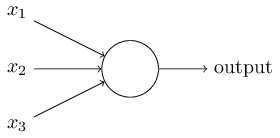
\includegraphics{perceptron.pdf}
	\caption{感知器模型}
	\label{perceptron}
\end{figure}

如图//所示,感知器接收若干个二进制输入$x_1, x_2, x_3, ...$并输出一个二进制结果。Rosenblatt 提出了一种计算感知机输出值的简易准则,他引入“权重(weight)”
的概念,用实数$w_1, w_2,...$来表示每个输入的重要性。最后神经元的输出,0 或者 1,是由加权和 $\sum_j w_{j}x_{j}$是否小于某个门限值决定的。和
权重一样,门限值也是神经元的一个实数参数。以上准则可由下面的公式\ref{eqn:perceptron}表示:
\begin{equation}
\label{eqn:perceptron}
output = \left\{ \begin{array} { l l } { 0 } & { \text { if } \sum _ { j } w _ { j } x _ { j } \leq \text { 门限 } } \\ { 1 } & { \text { if } \sum _ { j } w _ { j } x _ { j } > \text { 门限 } } \end{array} \right.
\end{equation}

以上就是感知器的简单数学模型。可以把感知器看成是一种对输入特征进行加权并输出决策的设备。可以结合实际举一个简单的例子。假如某人要决定周末是否
外出游玩,那么影响他决策的因素就可能是以下三个方面:

1. 天气是否晴好?

2. 是否有同伴陪同?

3. 游玩地点是否在地铁站附近?

我们可以用变量$x_1, x_2, x_3$来表征这三个二进制影响因素,比如$x_1 = 1$表示天气晴好,$x_2 = 1$表示有同伴陪同,$x_3 = 1$表示目标地点在地铁站
附近。

以上三个影响因素对最后的决定的影响程度是不一样的,这就需要对每个影响因素设置一个权重。假如天气是最关键的决定因素,在天气坏的情况下仍然出门的可能性很小,
那么就可将$x_1$对应的权重设置为$w_1=6$,其余两个影响因素的权重都设置为$w_2=1, w_3=1$。现在假如我们把门限值设置为 3,那么在天气坏的情况下,无论
其他两个因素是什么样的,最后的加权和都不会超过 3,从而做出周末不外出游玩这个决定。

通过设置不同的权重和门限,可得到不同的决策模型。比如将门限值降低可增加外出游玩的可能性,将是否有同伴陪同的权重提高可增加同伴对外出游玩与否的影响程度。

显然以上的感知器模型并不能完全体现人类决策的复杂性而只是一个简单的示例。通过堆叠多层感知器,可得到做出更加微妙决策的感知器网络。

\begin{figure}[h]
	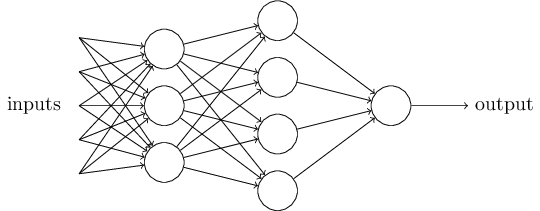
\includegraphics{layeredperceptron.pdf}
	\caption{多层感知器模型}
	\label{layeredperceptron}
\end{figure}

如图\ref{layeredperceptron},第一层感知器一共做出三项简单决策,这三项决策又接着输入到第二层的两个感知器得出两个更进一步的决策,最后这两个决策又输入到最后一个感知器得到
最后的决策。这种级联方式可以让后面的感知器得出比前面的感知器更抽象的结果,从而解决更加复杂的决策问题。

通过引入“偏置(bias)”$b$,公式\ref{eqn:perceptron}也可以改写为公式\ref{eqn:perceptronbias}:
\begin{equation}
	\label{eqn:perceptronbias}
output = \left\{ \begin{array} { l l } { 0 } & { \text { if } w \cdot x + b \leq 0 } \\ { 1 } & { \text { if } w \cdot x + b > 0 } \end{array} \right.
\end{equation}

偏置的概念可理解为输出 1 的容易程度。从生物学的角度也可说成神经元达到激发态的容易程度。偏置的引入可简化后面的公式表示。

\section{激活函数}
本节所介绍的激活函数的引入是为了使人工神经网络中感知器的权重和偏置的自动化训练成为可能。如果我们想通过调整感知器参数从而使网络的整体
表现满足某种特定需求,那么对感知器参数的微小改动必须也对应输出的微小改动,即稍稍改变权重和偏置不会导致输出的剧烈变化。前面的感知器模型只能输出0和1
两种结果,显然不能满足输出缓慢变化的特征。为了得到满足这种特征的感知器,需要对上节感知器模型做出修改,在输出时应用激活函数 $f$:
\begin{equation}
	\label{eqn:sigmoid}
	\sigma ( z ) \equiv \frac { 1 } { 1 + e ^ { - z } }
\end{equation}

即,对于输入$x_1, x_2, ...$,权重$w_1, w_2, w_3,...$ 和权重 $b$,sigmoid 神经元的输出是:
\begin{equation}
	\label{eqn:sigmoidoutput}
	\frac { 1 } { 1 + \exp \left( - \sum _ { j } w _ { j } x _ { j } - b \right) }
\end{equation}
从图\ref{sigmoid_step}可以看出,本质上 sigmoid 函数是阶跃函数的平滑版本,这也说明了为什么 sigmoid 激活函数的引入可以解决输出剧烈变化的问题。

\begin{figure}[htbp]
	\subfigure[]{
		\label{sigmoid}
		\includegraphics{sigmoid.pdf}}
	\subfigure[]{
		\label{step}
		\includegraphics{step.pdf}}
	\caption{Sigmoid 与阶跃函数对比图}
	\label{sigmoid_step}
\end{figure}

$\sigma$ 函数的重要性在于其平滑性,而与其具体的形状并没有太大的关系,$\sigma$ 的平滑度意味着权重中的微小变化
$\Delta w_j$ 和偏置中的 $\Delta w_j$ 将在神经元的输出中产生小的变化 $\Delta output$。
 事实上,微积分告诉我们 $\Delta output$ 很接近:
\begin{equation}
	\label{eqn:sigmoiddelta}
	\Delta \mathrm { output } \approx \sum _ { j } \frac { \partial \mathrm { output } } { \partial w _ { j } } \Delta w _ { j } + \frac { \partial \text { output } } { \partial b } \Delta b
\end{equation}

$\sigma$ 函数并不是唯一的激活函数形式,常用的激活函数还有 ReLU 激活函数。此函数是一个分段线性函数:
\begin{equation}
	\label{eqn:relu}
	\operatorname { ReLU } ( x ) = \left\{ \begin{array} { l l } { x } & { \text { if } x > 0 } \\ { 0 } & { \text { if } x \leq 0 } \end{array} \right.
\end{equation}

函数图像是:
\begin{figure}[htbp]
	\includegraphics{relu.pdf}
	\caption{ReLU 激活函数图像}
	\label{relu}
\end{figure}

从公式\ref{eqn:relu}和图\ref{relu}可以观察到 ReLU 函数把所有的负值都变为0,而正值线性变化,这种操作叫做单侧抑制。
尤其体现在深度神经网络模型(如CNN)中,当模型增加N层之后,理论上 ReLU 神经元的激活率将降低2的N次方倍。
相对于 sigmoid 函数,ReLU 能更好地实现网络模型的稀疏性,同时也符合近年来神经科学对神经元工作稀疏性的研究【引用】,同时 ReLu 在
正区间梯度总是为定值的特性也有利于避免梯度消失问题。

\section{神经网络结构}
单个感知器或者说人工神经元只是生物神经细胞的近似理
想化实现,功能更加简单。要想模仿人类的神经系统的推理运算功能,需要多个人工神经的协调配合实现高阶的抽象能力
并完成复杂的功能。通过特定的连接或信息传递方式进行配合的神经元可以看作是一个网络,我们称之为人工神经网络。

\begin{figure}[htbp]
	\includegraphics{ann_structure.pdf}
	\caption{神经网络一般结构}
	\label{ann_structure}
\end{figure}

图\ref{ann_structure}给出了人工神经网络的一般结构。人工神经网络一般由多层感知器级联而成。第一层感知器,也就是图中的最左边那层称为
输入层,它的作用是将输入数据传递到网络中。最后一层感知器被称为输出层,也就是图中的最右那层,用来得到网络的计算结果。
而输入层和输出层之间的各层统称为隐含层(hidden layer),隐含的意思是这些神经元处于神经网络内部,不与外部直接进行
信息交换。上图中的隐含层层数为 2,不过隐含层的层数也可以是任意正整数。历史上这类简单的多层神经网络也被成为多层感知机
(multilayer perceptrons)。

目前所提到的神经网络结构都是不包含反馈结构的,即所有网络层的输入都来自于上一层的输出,这种网络结构被称为前馈神经网络
(feedforward neural networks)。另外一种神经网络类型包含循环结构,即存在某些层的输出又作为前面网络层输入的情况,这种
网络结构统称为循环神经网络(recurrent neural networks)。循环神经网络在时序信号的处理,如语音识别领域,取得了良好
的效果。

\begin{figure}[htbp]
	\includegraphics{rnn_structure.pdf}
	\caption{循环神经网络}
	\label{rnn_structure}
\end{figure}

前馈神经网络是应用最广泛的神经网络模型,性能良好,也比较易于实现与调参,本文后面章节在处理探地雷达信号目标识别问题
时使用的卷积神经网络也属于前馈神经网络的一种。

\section{反向传播算法}
在将神经网络应用到分类和回归任务时,神经网络的预测性能由每层各神经元的权重和偏置组成的参数矩阵决定。神经网络的训练过程
即用特定的优化方法调整参数矩阵,使神经网络能特定的输入产生我们期望的输出。

对于一个前馈神经网络,我们使用下面的方法标记各参量。用 $L$:表示神经网络的层数;用$m^{(l)}$表示第$l$层神经元的个数;用
$f_l ()$ 表示$l$层的激活函数;$W ^ { ( l ) } \in \mathbb { R } ^ { m ^ { ( l ) } \times m ^ { l - 1 } }$ 用来表示
$l-1$ 层到 $l$ 层的权重矩阵;$\mathbf { b } ^ { ( l ) } \in \mathbb { R } ^ { m ^ { l } }$ 表示偏置矩阵;
$\mathbf { z } ^ { ( l ) } \in \mathbb { R } ^ { m ^ { l } }$ 表示$l$层神经元的净输入;$\mathbf { a } ^ { ( l ) } \in \mathbb { R } ^ { m ^ { l } }$
表示$l$层神经元的输出。

则我们可以用以下公式描述信息在前馈神经网络中的传播过程:
\begin{equation}
	\label{eqn:qiankuichuanbo1}
	\mathbf { z } ^ { ( l ) } = W ^ { ( l ) } \cdot \mathbf { a } ^ { ( l - 1 ) } + \mathbf { b } ^ { ( l ) }
\end{equation}
\begin{equation}
	\label{eqn:qiankuichuanbo2}
	\mathbf { a } ^ { ( l ) } = f _ { l } \left( \mathbf { z } ^ { ( l ) } \right)
\end{equation}

\ref{eqn:qiankuichuanbo1} 与 \ref{eqn:qiankuichuanbo2} 也可以合并为:
\begin{equation}
	\label{eqn:qiankuichuanbo3}
	\mathbf { z } ^ { ( l ) } = W ^ { ( l ) } \cdot f _ { l - 1 } \left( \mathbf { z } ^ { ( l - 1 ) } \right) + \mathbf { b } ^ { ( l ) }
\end{equation}

或者:
\begin{equation}
	\label{eqn:qiankuichuanbo4}
	\mathbf { a } ^ { ( l ) } = f _ { l } \left( W ^ { ( l ) } \cdot \mathbf { a } ^ { ( l - 1 ) } + \mathbf { b } ^ { ( l ) } \right)
\end{equation}

由此可以得到数据在更层传播的路径 \ref{eqn:qiankuichuanbo5},将向量 $\mathbf{x}$ 作为第 1 层的输入经过逐次传播后可得到将整个网络看成一个整体的
复合函数 $\phi(\mathbf{x} ; W, \mathbf{b})$
,其中 $L$ 表示总层数。
\begin{equation}
	\label{eqn:qiankuichuanbo5}
	\mathbf{x}=\mathbf{a}^{(0)} \rightarrow \mathbf{z}^{(1)} \rightarrow \mathbf{a}^{(1)} \rightarrow \mathbf{z}^{(2)} \rightarrow \cdots \rightarrow \mathbf{a}^{(L-1)} \rightarrow \mathbf{z}^{(L)} \rightarrow \mathbf{a}^{(L)}=\varphi(\mathbf{x} ; W, \mathbf{b}) )
\end{equation}

1989 年,Cybenko 等人的研究证明【引用】,上述前馈神经网络所表征的 $\phi(\mathbf{x} ; W, \mathbf{b})$ 函数在隐含神经元足够多的情况下,可以无限
你和任意的连续非线性函数。这说明神经网络具有通用近似能力,这也是用神经网络来解决机器学习问题的理论基础。

对于分类问题,还需要将 $\phi$ 函数作为某种分类器的输入,从而得到每种类别的概率。
\begin{equation} 
\hat{y}=g(\varphi(\mathbf{x}), \theta)
\end{equation}
其中,$\hat{y}$ 为每类的概率输出,$\theta$ 为分类器的参数,$g$ 为分类器。

对于多分类问题,常用的分类器为 Softmax 分类器。对于具有$N$个分类的多分类问题,式\ref{eqn:softmax}给出了 softmax 函数的定义。softmax 函数可以
将一组 $\phi$ 给出的输出转化为一组总和为1的概率,并且不影响转化前的大小相对关系。通过分类器的归一化之后的概率输出便可得出最可能的预测,因此分类器
基本上位于网络的最后一层。
\begin{equation} 
\label{eqn:softmax}
\operatorname{softmax}\left(s_{i}\right)=\frac{e^{s_{i}}}{\sum_{j=1}^{N} e^{s_{j}}} \quad(i=1, \cdots, N)
\end{equation}

上面说明了数据在前馈神经网络中正向传播的过程。为了使神经网络得到可靠的预测结果,需要对网络的参数,包括各层的权值和偏置,进行训练。训练一般采用
梯度下降算法,梯度下降时需要一个评估模型预测性能的损失函数。损失函数一般由模型预测结构和真实结构的交叉熵计算得出。交叉熵由式\ref{eqn:cross_entrophy}定义。
\begin{equation}
\label{eqn:cross_entrophy} 
\mathcal{L}(\mathbf{y}, \hat{\mathbf{y}})=-\mathbf{y}^{\mathrm{T}} \log \hat{\mathbf{y}}
 \end{equation}
其中$\mathbf{y}$与$\hat{\mathbf{y}}$分别表示实际标签与预测结果。

在交叉熵的基础上还可以定义风险函数:
\begin{equation} 
\mathcal{R}(W, \mathbf{b})=\frac{1}{N} \sum_{n=1}^{N} \mathcal{L}\left(\mathbf{y}^{(n)}, \hat{\mathbf{y}}^{(n)}\right)+\frac{1}{2} \lambda\|W\|_{F}^{2}
\end{equation}
\begin{equation} 
=\frac{1}{N} \sum_{n=1}^{N} \mathcal{L}\left(\mathbf{y}^{(n)}, \hat{\mathbf{y}}^{(n)}\right)+\frac{1}{2} \lambda\|W\|_{F}^{2}
\end{equation}
其中$\mathbf{W}$和$\mathbf{b}$分别表示网络中的权重和偏置;其中$\|W\|_{F}^{2}$为了防止过拟合现象而引入的正则化项;$\lambda$是为正数的参数。
这里的正则化项一般由Frobenius范数(式\ref{eqn:frobenius})给出:
\begin{equation} 
\label{eqn:frobenius}
\|W\|_{F}^{2}=\sum_{l=1}^{L} \sum_{i=1}^{m^{(l)}} \sum_{j=1}^{(l-1)}\left(W_{i j}^{(l)}\right)^{2}
\end{equation}

对模型的训练过程即调整模型参数使得风险函数最小的过程。按照梯度下降原理,每次迭代过程中第$l$层
的参数更新公式为:
\begin{equation} 
\begin{aligned} W^{(l)} & \leftarrow W^{(l)}-\alpha \frac{\partial \mathcal{R}(W, \mathbf{b})}{\partial W^{(l)}} \\ &=W^{(l)}-\alpha\left(\frac{1}{N} \sum_{n=1}^{N}\left(\frac{\partial \mathcal{L}\left(\mathbf{y}^{(n)}, \hat{\mathbf{y}}^{(n)}\right)}{\partial W^{(l)}}\right)+\lambda W^{(l)}\right) \\ \mathbf{b}^{(l)} & \leftarrow \mathbf{b}^{(l)}-\alpha \frac{\partial \mathcal{R}(W, \mathbf{b})}{\partial \mathbf{b}^{(l)}} \\ &=\mathbf{b}^{(l)}-\alpha\left(\frac{1}{N} \sum_{n=1}^{N} \frac{\partial \mathcal{L}\left(\mathbf{y}^{(n)}, \hat{\mathbf{y}}^{(n)}\right)}{\partial \mathbf{b}^{(l)}}\right) \end{aligned}
\end{equation}
式中的$\alpha$代表学习率。


\section{卷积神经网络}
上节所述传统的前馈神经网络一般采用全连接结构,即每层所有神经元的输出都与下层的每一个神经元相连,也就是每一个连接都尤其对应的权重参数。
随着网络层数的增加,网络模型中参数的数量也将急剧增加。这样将会导致两个问题,一是参数过多时导致模型训练时计算量过大训练效率低,二是过多的
参数很容易导致过拟合现象即网络模型不能正确提取数据中的关键特征而过分强调无关细节。

在图像处理领域,以上所述问题尤其严重,因为相比于一维信号,图片数据需要用二维矩阵来表示,数据量大。特别是在图片为彩色的情况下,对于红、绿、
蓝三个通道,都要对应一个二维矩阵,这又使数据成倍增加。另外,对于图像处理来说,有很多图像上的特征在局部都是不变的,如材质的纹理,人脸的五官等,如果使用
全连接网络则很难提取出这些局部的特征。

卷积神经网络就是针对以上两个问题提出的一种改进型神经网络结构,可以很好地应用于图像和视频的各种图像分类、物体识别、图像分割等问题。如前面章节
所述,探地雷达的回波信号是发射天线产生的电磁波脉冲在地层中的反射传到接收天线并通过接收机与采集板回传到PC端信号采集软件的一维实数信号,也就是
所谓的A扫。随着收发天线的移动,不断采集到的二维信号可组合形成 B 扫数据。B 扫数据在形式上可看成是一种图像数据,另外,雷达B扫图像中目标反射所
形成的类似于双曲线图像也有明显的局部化特征。虽然反射特征在整体B扫中的位置是不确定的,但是在每个反射特征的周围一块区域却存在着相似的特性。考虑到
以上特点,探地雷达数据符合卷积神经网络的应用领域和数据特点。本文后面章节将使用卷积神经网络对探地雷达目标识别问题进行处理,并与多层感知机的效果作
对比。

卷积神经网络是受生物学上感受野的机制而提出。感受野(receptive field)主要是指听觉、视觉等神经系统中一些神经元的特性,即神经元只接受其所支
配的刺激区域内的信号。在视觉神经系统中,视觉皮层中的神经细胞的输出依赖于视网膜上的光感受器。视网膜上的光感受器受刺激兴奋时,将神经冲动信
号传到视觉皮层,但不是所有视觉皮层中的神经元都会接受这些信号。一个神经元的感受野是指视网膜上的特定区域,只有这个区域内的刺激才能够激活该
神经元。

应用到机器学习领域。卷积神经网络主要用到了三个基本思想:局部感受野、权值共享和子采样。下面分别对这三种思想作阐述。

【局部感受野】

前面所述全连接前馈神经网络中,输入数据是一维的列向量。在卷积神经网络中输入是以多维的形式组织的.

和前面的网络类似,输入层数据也要连接到隐含层的神经元上,不过在卷积神经网络中,我们不会将每个输入都连接到每一个隐含层神经元上。
反之我们只会连接一小部分局部的输入数据。更精确地说,第一个隐含层的每一个神经元都会连接到输入神经元的一小块区域,比如说一个5x5
尺寸的正方形区域(共25个输入数据)。这种连接方式可由图\ref{perception_filed}来说明(图中没有画出所有的输入神经元到隐含层神经元的连接)。

\begin{figure}[htbp]
	\includegraphics{perception_field.pdf}
	\caption{卷积层连接方式}
	\label{perception_filed}
\end{figure}

上述正方形区域被称为隐含神经元的局部感受野。局部感受野可看成作用在输入数据上一个窗。每一个从局部感受野到对应隐含神经元的连接都包含一个
权重,另外这个对应的隐含神经元本身也会有一个偏置参量。

将代表局部感受野的正方形窗在输入数据上平移,同时平移对应的隐含神经元,我们即可将所有的局部感受野与隐含神经元连接起来。

【权值共享】

上面提到局部感受野到隐含神经元的每一个连接都包含一个权重,此权重可以由一个矩阵$\mathbf{w}$来表示,这个矩阵的尺寸与局部感受野的尺寸相同。
但是在这里有一个值得注意的地方,即对于卷积神经网络从输入层到隐含层的每一个权重矩阵都是共享的。权重共享的目的是解决局部特征的学习问题,
因为权重共享之后,在二维数据某一位置学习到的特征也可应用到二维数据的其他位置。应用权重共享之后,对于位置为$j$,$k$的隐含层神经元,其输出是:
\begin{equation} 
\label{eqn:cnn_hidden_neuron}
f\left(b+\sum_{l=0}^{k} \sum_{m=0}^{k} w_{l, m} a_{j+l, k+m}\right)
\end{equation}
其中,$f$ 是激活函数,$b$ 是共享的偏置,$w_{l,m}$ 是共享的权重矩阵,$a_{j+l,k+m}$ 是对应的感受野输入,$k$ 是感受野尺寸。同时这里还要指出,
式\ref{eqn:cnn_hidden_neuron}中的求和部分可能看成是一个二维卷积的过程,这也就是卷积神经网络名称的由来。

从输入层到隐含层的映射被称为特征映射,即此映射包含了从输入数据中学习到的一般特征。在卷积神经网络术语中,共享的权重矩阵
$\mathbf{w}$和偏置$b$又被称为“核”或者“滤波器”。一般情况下,单个特征映射无法满足抽象出数据中足够多二维特征的要求。
所以在实际应用中,输入层可以映射到多个并列的隐含层,其中每一个隐含层都对应一个独立的特征映射及滤波器。

【子采样】

上面包含卷积运算的隐含层叫做卷积层。除了卷积层,卷积神经网络中还包含汇聚层(pooling layer)。汇聚层的作用是对卷积层输出的数据做
简化,也就是子采样,它通常紧接着卷积层使用。汇聚层将隐含层的输出结果矩阵划分成一批重叠或者不重叠的区域,然后对每个区域应用汇聚函数
得到一个单个的值,这样做实质上就是把隐含层的输出结果尺寸减小,即子采样的过程。常用的汇聚函数有最大汇聚和平均汇聚两种,分别可以表示为
\ref{eqn:max_pooling} 与 \ref{eqn:mean_pooling}。
\begin{equation}
\label{eqn:max_pooling} 
Y_{m, n}^{d}=\max _{i \in R_{m, n}^{d}} x_{i}
\end{equation}
\begin{equation} 
\label{eqn:mean_pooling}
Y_{m, n}^{d}=\frac{1}{\left|R_{m, n}^{d}\right|} \sum_{i \in R_{m, n}^{d}} x_{i}
\end{equation}
使用汇聚层之后,可以在大大减少神经元的数量的同时使神经网络对于一些微小细节的改变保持不敏感性,避免过拟合的发生。

如图\ref{cnn_structure}所示,卷积层、汇聚层和全连接层一起构成一个典型的卷积神经网络。一个卷积块为连续M 个卷积层和b个汇聚层(M
通常设置为 2 $\sim$ 5, b为 0或 1)。一个卷积网络中可以堆叠 $N$ 个连续的卷积块,
然后在接着 K 个全连接层($N$ 的取值区间比较大,比如 1 $\sim$ 100或者更大;$K$
一般为0 ~ 2)。
\begin{figure}[h]
	\includegraphics{cnn_structure.pdf}
	\caption{卷积神经网络结构示意图}
	\label{cnn_structure}
\end{figure}

按照图\ref{cnn_structure}给出的连接方式,结合实际问题的特点,不断增加网络的层数,达到足够提取出数据中的抽象特征进行高准确度预测
的效果,这样的网络被称为深度卷积网络。由于深度卷积网络可以利用数据的二维结构,而且所需要训练的参数相对来说更少,因此它是目前深度
学习领域中应用较为广泛的网络结构。

\section{本章小结}

